\chapter{跨卷综合算例}\label{v0ch:29}
\begin{chaptersummary}
前面分别讨论了离散算子、代数算法和执行成本，本章通过可复现实验将三者重新连接。各案例先核验模型、误差与约束，再记录求解和数据移动的成本。以相同问题和目标误差比较总时间，可以将局部核函数分析转化为跨卷的完整计算决策。
\end{chaptersummary}
\learninggoals{建立统一实验记录；完成 Maxwell 与高阶输运案例；区分核基准、完整求解与跨模型比较。}
\paragraph{核心问题}怎样确认更快的程序仍解决了同一个问题？

\section{Krylov 与 AMG：从 Poisson 到预条件}
从第一卷的空间离散取二维 Dirichlet Poisson。先以已知解构造右端，确认直接法、CG 与预条件解的真实残差；再用解析连续解比较离散误差。记录自由度、$\nnz$、排序、因子填充、预条件构造、迭代、时间与误差。
采用代数制造右端 $\bm b=A\bm x_*$ 检查线性求解器，再以连续解析解检验 PDE 收敛阶，代码分别记录这两层误差。多右端实验复用相同因子，展示构造成本的摊销；两层 AMG 例则用于核验粗空间与修正机制。
Krylov 成本应拆成 SpMV、预条件、点积与正交化；AMG 则逐层记录平滑、限制、粗解与插值。小规模上，减少迭代未必抵消构造和 Python 调用成本；大规模上，粗层通信和全局归约又可能改变排序。教学例实测的是串行层次作用，分布式 AMG 的粗层扩展仍需独立实验。
\section{完整 Maxwell 推进}
取周期单位立方体、真空 $c=1$，右行横波
\[
 E_y(x,t)=\sin(2\pi(x-t)),\qquad B_z(x,t)=\sin(2\pi(x-t)).
\]
其他分量为零。分别在各自空间点和 $t=-\Delta t/2$ 初始化磁场，选
$\Delta t\le\nu h$、$\nu<1/\sqrt3$，最后一步统一调整以精确到达相同 $T$。比较两组网格上的 $L^2$ 误差、数值相位、步数和时间；初值不能把半时间层误当整层。
CPU 程序还从随机边场计算离散旋度并检验散度，监测完整推进中的 $\diverg_h B$ 与修正能量。无源电场散度检验对应零电荷；有源推广需相容电流和连续性更新。
\begin{figure}[htbp]\centering
\IfFileExists{Vol0_Linear_Algebra_HPC/figures/convergence.pdf}{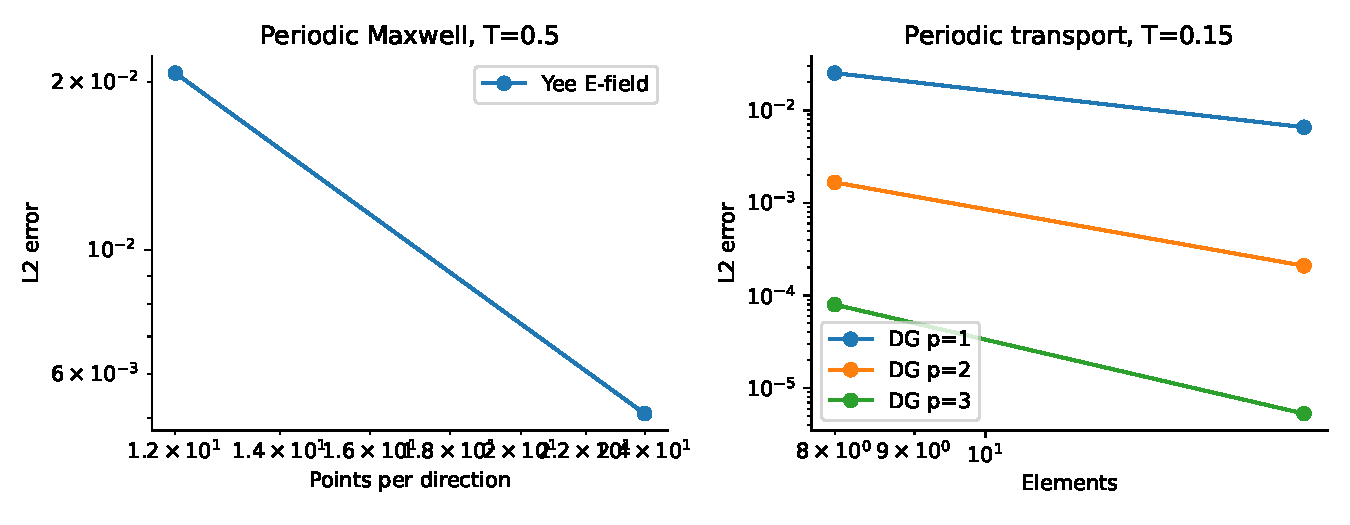
\includegraphics[width=.88\textwidth]{Vol0_Linear_Algebra_HPC/figures/convergence.pdf}}{}
\caption{本卷 CPU 程序生成的实际收敛数据：Yee 横波与周期输运。误差定义和参数见结果记录。}
\end{figure}
从 CPU 扩展到 GPU 时保留 SoA、两相顺序和初值；扩展到 MPI 时按每相交换所需分量，再做内部与边界更新。附带 CUDA 全场程序提供设备端链路，MPI 全场程序包含每相 halo 和全局约束诊断。附录与实验数据记录执行范围，跨节点与多 GPU 耦合则按同一误差和约束口径继续测量。
\section{完整高阶 DG 与 FR 接口}
对 $u_t+u_x=0$、周期 $u(x,0)=\sin(2\pi x)$，在各单元用 Legendre 模态
$u_h=\sum_{m=0}^{p}\widehat u_mP_m(\xi)$。弱形式为
\[
 \frac h2 M\dot{\widehat{\bm u}}
 =S\widehat{\bm u}-\bm\phi(1)\widehat f_R
                         +\bm\phi(-1)\widehat f_L,\quad
 M_{mm}=\frac2{2m+1},\quad S_{m\ell}=\int_{-1}^{1}P'_mP_\ell.
\]
正速度上风通量取左侧迹。体算子、面通量和对角质量逆均可直接实现。代码采用 RK4 和保守步长，比较 $p=1,2,3$ 与不同单元数的误差、自由度、步数及时间。
FR 接口实验在 $p=1$ Lobatto 两端点上，用
$g_L=(P_2-P_1)/2$、$g_R=(P_2+P_1)/2$
构造导数修正，核验它与同一精确质量及求积约定下的 nodal DG 算子等价。改变校正函数后，再比较相应提升与体积算子。三维张量导数另与稠密 Kronecker 作用对照，用于检查和因子分解。
MPI 版本按单元划分，每个 RK 阶段交换上风迹，质量逆保持单元局部。GPU 优化可将多个同阶单元批量化，复用导数矩阵并分离体项与面项；阶数增大同时提高寄存器需求和体面比。当前 GPU 可执行验证覆盖 Yee 与布局，完整 DG 的 GPU 移植作为单列扩展任务。
\conceptbridge{为什么核函数吞吐更高，完整 DG 模拟仍可能更慢？}{高阶局部运算提高算术强度，也改变时间步约束、每步阶段和误差。只有减少达到目标精度所需的总单元与总步数，局部吞吐优势才可能转化为端到端收益。}{核复用 $\longrightarrow$ 精度与稳定步长 $\longrightarrow$ 物理终止时间成本。}
\section{FDM、FVM、FEM 与 LBM 的访问对照}
同一周期输运问题还包含一阶上风 FVM，可与 DG 比较误差和总时间。FDM 七点算子、Yee、DG 张量、LBM 迁移碰撞及 CSR/GEMM 则分别展示不同访问模式。跨模型的格点更新率用于分析实现指纹，方法选型则以共同物理问题与目标误差为依据。
FEM 用装配矩阵与局部矩阵自由作用的一致性验证接口；FVM/DG 面通量检查守恒，LBM 检查周期总质量。每种实现先验收，再计时。
\subsection{规则 stencil 与交错 stencil}
七点 FDM 每次输出一个标量场；Yee 每整步更新六个交错分量并分两相读取。二者都可采用空间连续索引和 halo，但相同格点数并不表示相同自由度或相同物理问题。分别比较 8 FLOPs 的 Laplacian、42 FLOPs 的差分型 Yee 与 30 FLOPs 的融合型 Yee，并注明访问模型。
\subsection{邻接表、非规则访问与几何}
FVM 案例将非均匀周期单元重新编号，用面左右单元索引读取状态、计算通量并累加残量。验证置换前后的结果一致，且体积加权残量和为零。该例隔离编号与 gather/scatter；一般非结构网格还需面法向、面积、重构邻域和图分区。MPI 交换应由跨分区面确定，而不是假定每个单元都有固定数组邻点。
\subsection{局部矩阵与人口分布布局}
一维 P1 FEM 比较 CSR 作用与逐单元差分累加，检查同一边界消元后的输出。LBM 则分别计时迁移、碰撞和完整步：迁移布局实验验证 push/pull 及 AoS/SoA 输出相同，完整周期 BGK 实验核验总质量。GPU occupancy 还受碰撞活跃变量与边界分支影响，单个 CPU 布局测试无法预测该量。
\paragraph{八组案例的对应关系}
FDM--Yee 的 stencil 对照、FVM 邻接、DG/FR 体面结构、LBM 迁移碰撞、Krylov、AMG、完整 Maxwell 和完整高阶 DG 分别覆盖本卷的八个性能接口。各自的数值验收与执行范围在代码和附录中记录。
\section{统一验收与选择}
\begin{center}\small
\begin{tabularx}{\textwidth}{lX}
\toprule 维度&应记录内容\\\midrule
物理与离散&方程、边界、初值、$T$、网格、阶数、自由度\\
数值准确性&空间/时间误差、相位、真实残差、守恒与约束\\
算法工作&时间步、阶段、迭代、预条件与层次复杂度\\
资源&数组/因子内存、模型 FLOPs、模型流量、消息与归约\\
执行范围&构造、推进、传输、通信、验证及输出是否计入\\\bottomrule
\end{tabularx}
\end{center}
\costnote{固定自由度比较用于分析实现，固定误差比较用于选择方案；两种实验都应报告。附带小规模 CPU 测试验证流程，大规模优化还需真实工作集、并行规模与硬件计数器。}
\coderef{run_all.py; run_accelerators.py; fdtd/yee.py; dg_fr/transport.py}
\aiexercise{运行本卷实验，从 JSON 生成误差--时间与误差--自由度图。先检查每条曲线的物理问题、终止时间和误差范数是否一致。}{选择一个误差阈值，为 Yee 或 DG 设计网格、阶数和时间步联合搜索；将构造、通信与输出纳入端到端预算。}
\studyroute{跨节点硬件基准与工程级复杂边界应用留待进一步实验，复现命令和计时约定见实验指南。参考 \cite{yee,hesthaven,roofline}。}{verification versus validation; manufactured solution; error versus cost; constraint preservation; time to solution}
